\documentclass[9pt,xcolor=pdftex,dvipsnames,table]{beamer} 
\setbeamercolor{bgcolor}{fg=white,bg=blue!100}
\mode<presentation>
{
  \usetheme{Darmstadt}
 \setbeamertemplate{navigation symbols}{}
  \setbeamercovered{transparent}
  \setbeamertemplate{footline}
{\rightline{\insertframenumber/\inserttotalframenumber}}
}

\def\newblock{}

\newenvironment{changemargin}[2]{% 
  \begin{list}{}{% 
    \setlength{\topsep}{0pt}% 
    \setlength{\leftmargin}{#1}% 
    \setlength{\rightmargin}{#2}% 
    \setlength{\listparindent}{\parindent}% 
    \setlength{\itemindent}{\parindent}% 
    \setlength{\parsep}{\parskip}% 
  }% 
  \item[]}{\end{list}} 
  
\usepackage[english]{babel}
\usepackage{amsmath}
\usepackage{lipsum}
\usepackage[latin1]{inputenc}
\usepackage{times}
\usepackage[latin1]{inputenc}
\usepackage{tipa}
\usepackage{color}
\usepackage{booktabs}
\usepackage{colortbl}
\usepackage{movie15}
\usepackage{gb4e}
\usepackage{longtable}
\usepackage{pgf,pgfarrows,pgfnodes}
\usepackage{tikz} 
\usepackage{textpos}            % free image positioning 
\setlength{\TPVertModule}{1cm}  % unit for vertical positioning 
\setlength{\TPHorizModule}{1cm} % unit for horizontal positioning 

\definecolor{lightorange}{rgb}{1,0.75,.25}
\definecolor{lightred}{rgb}{1,0.25,.25}
\definecolor{lightblue}{rgb}{.25,.25,1.0}
\definecolor{lightgray}{rgb}{.75,.75,.75}

\usepackage[T1]{fontenc}

\title{How To Wreck a Nice Beach}
\author{Linguistics 409 $\cdot$ Computational Linguistics}
\date{}
\usepackage{gb4e}

\usepackage{natbib}
\bibliographystyle{apalike}

\makeatletter
\newcommand\textsubscript[1]{\@textsubscript{\selectfont#1}}
\def\@textsubscript#1{{\m@th\ensuremath{_{\mbox{\fontsize\sf@size\z@#1}}}}}
\newcommand\textbothscript[2]{%
  \@textbothscript{\selectfont#1}{\selectfont#2}}
\def\@textbothscript#1#2{%
  {\m@th\ensuremath{%
    ^{\mbox{\fontsize\sf@size\z@#1}}%
    _{\mbox{\fontsize\sf@size\z@#2}}}}}
\def\@super{^}\def\@sub{_}
\makeatother

\begin{document}
\definecolor{grey}{rgb}{1,0.6,.7}

\section{Introduction}

\begin{frame}

	\titlepage
	\vspace{-1.5cm}
	\begin{center}
    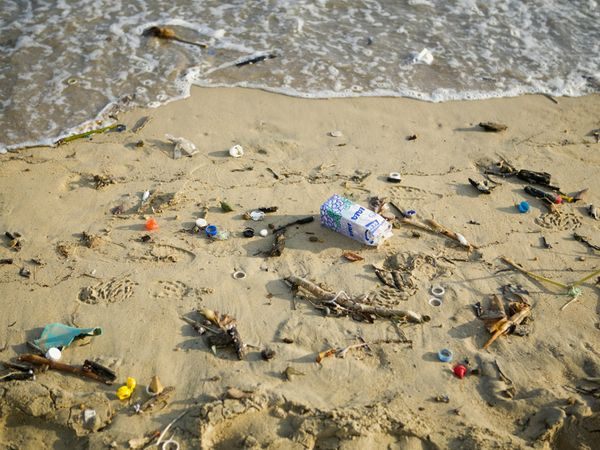
\includegraphics[scale=.38]{niceBeach.jpg}
	\end{center}
	
\end{frame}

\subsection{}
\begin{frame}{Relevant XKCD (802)}

	\begin{center}
    \includegraphics[scale=.2]{ASRXKCD}
	\end{center}
	
\end{frame}

\subsection{}
\begin{frame}{Relevant XKCD (802)}

	\begin{center}
    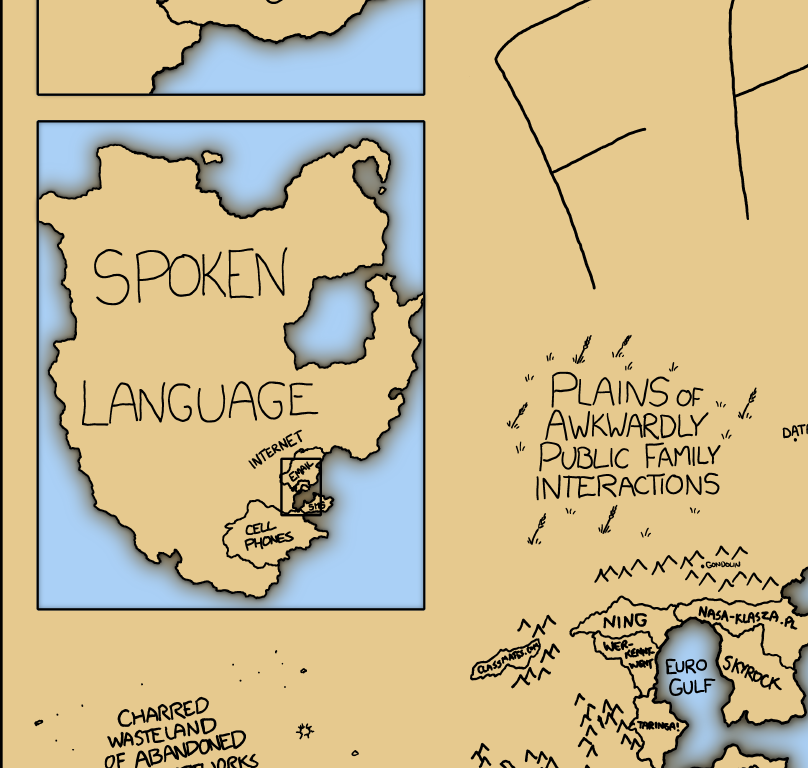
\includegraphics[scale=.75]{ASRXKCD-zoom}
	\end{center}
	
\end{frame}

\subsection{}
\begin{frame}{What is ASR?}
    \setbeamercovered{invisible}

{\large Speech-to-Text Transcription }
	\begin{itemize}
		\item Transform recorded audio into a sequence of words
		\item Just the words, no meaning...\pause
		\item But: ``Will the new display recognise speech?'' vs ``Will the nudist play wreck a nice beach?''
		\item Paralinguistic aspects: how did they say it? (timing, intonation, voice quality)
	\end{itemize}
\end{frame}

\subsection{}
\begin{frame}{What isn't ASR?}
    \setbeamercovered{invisible}

{\large Speech-to-Text Transcription }
	\begin{itemize}
		\item Speaker diarization: Who spoke when?
		\item Speech recognition: what did they say?
		\item Language identification: what language are they speaking?
		\item Automatic Speech Understanding
	\end{itemize}
\end{frame}

\subsection{}
\begin{frame}{What is ASR?}

\begin{itemize}
	\item {\Huge How would automated speech recognition be useful?} \\ \pause
	\vspace{.25cm}
	\item {\Huge What applications have you used?} \\ \pause
	\vspace{.25cm}
	\item {\Huge What are some potential applications?}
\end{itemize}

\end{frame}

\subsection{}
\begin{frame}{Why is ASR so difficult?}

\begin{itemize}
	\item {\Huge What makes ASR so difficult?} \\ \pause
\end{itemize}

\begin{itemize}
	\item Fish tale
	\item Sinewave speech
	\item Indexical/socioindexical variation
	\item Intra-speaker variation
	\item Context-appropriate variation
	\item Allophonic variation
	\item but there is something deeper that makes ASR a strange task...
\end{itemize}

\end{frame}

\subsection{}
\begin{frame}{}

	\begin{center}
    \includegraphics[scale=.2]{ASRXKCD}
	\end{center}
	
\end{frame}w

\subsection{}
\begin{frame}{Why is ASR so difficult?}

{\large Sources generally recognized within CS/NLP: }
\vspace{.25cm}

\begin{description}
	\item[Size] Number of word types in vocabulary, perplexity
	\vspace{.25cm}
	\item[Speaker] Tuned for a particular speaker, or speaker-independent? Adaptation to F0, formants, indexical properties, socioindexical properties, but also unigram, bigram and trigram probabilities, habitual prosodic patterns, etc.
		\vspace{.25cm}
	\item[Environment] Acoustic environment includes noise, competing talkers, and so-called channel conditions (microphone, phone connection, room acoustics, etc.)
		\vspace{.25cm}
	\item[Style] Continuously spoken or isolated? Planned monologue or spontaneous conversation?  Human to human speech or Human to (idiot) computer speech?
\end{description}

\end{frame}

\section{Statistical ASR}
\subsection{}
\begin{frame}{Theory follows engineering here...}

\begin{itemize}
	\item Speech perception is one of the few fields in mainstream linguistics that has really embraced the findings of computational linguistics.
	
	\item ASR researchers realized long ago that intense effort is needed to derive and encode linguistic rules that accurately model speech
	\item And even then the model is not very good...
\end{itemize}

\begin{block}{Famous Quote attributed to Fred Jelinek circa 1988}
\vspace{.25cm}
 \begin{flushright}
{\Huge``Every time I fire a linguist,}\\{\LARGE the performance of the speech recognizer goes up''}
 \end{flushright}
 \vspace{.25cm}
\end{block}
\end{frame}

\subsection{}
\begin{frame}{Peterson \& Barney 1952}

	\begin{center}
    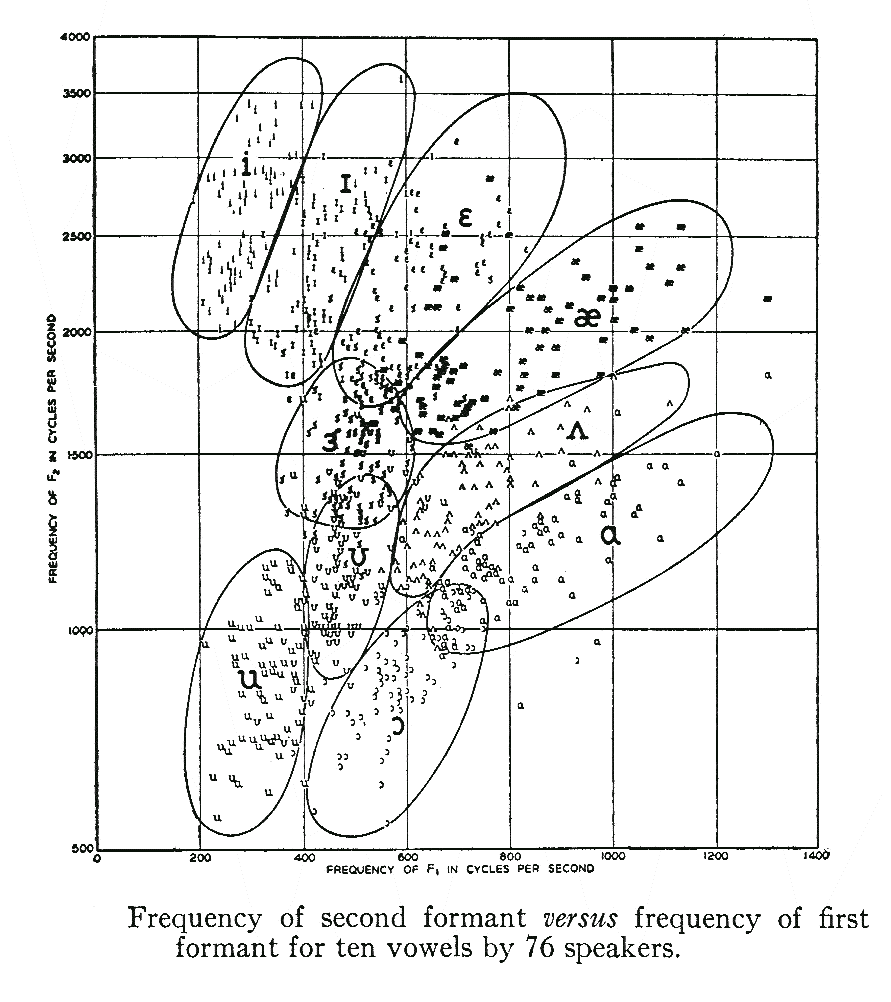
\includegraphics[scale=.2]{PetersonBarney52}
	\end{center}
	
\end{frame}

\subsection{}
\begin{frame}{Peterson \& Barney 1952}

	\begin{center}
    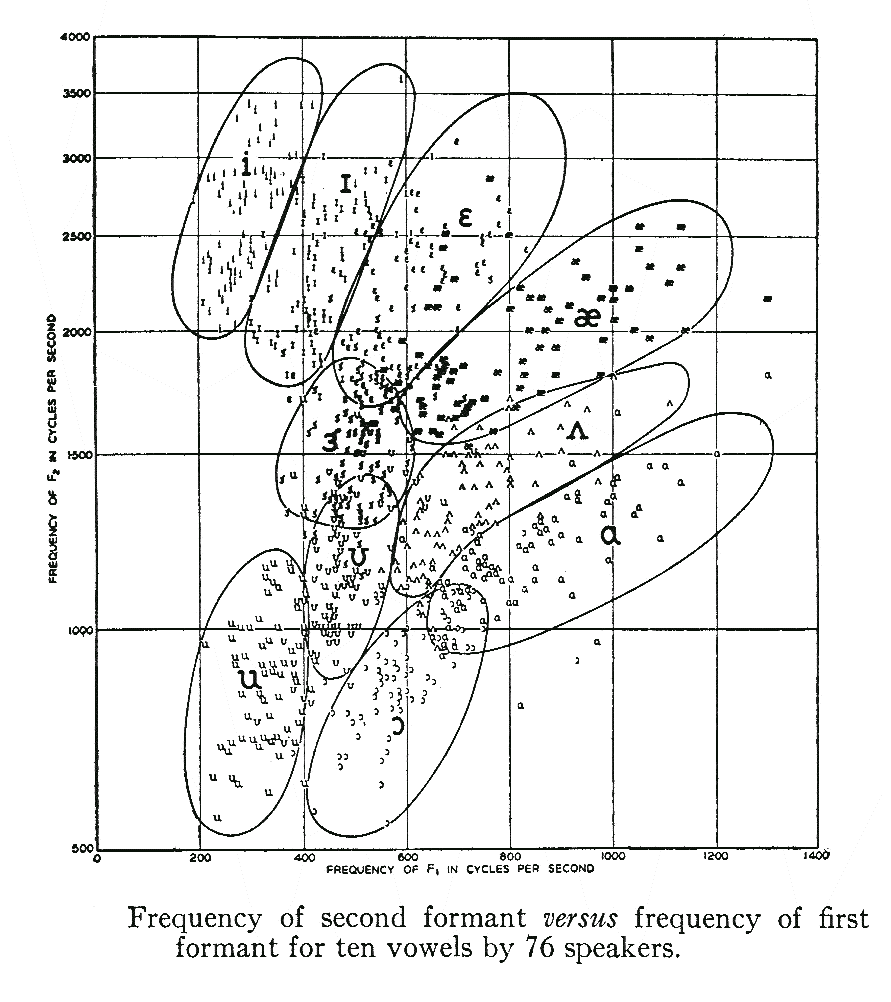
\includegraphics[scale=.5]{PetersonBarney52}
	\end{center}
	
\end{frame}

\subsection{}
\begin{frame}{Theory follows engineering here...}

\begin{itemize}
	\item It is very difficult to take account of the variability of spoken
language with, say, derivational phonology (which is not to say that people didn't try!)

	\item Data-driven machine learning approach: Construct simple models of
speech which can be learned from large amounts of data (thousands of hours of speech recordings)

	\item See, for example, exemplar theories of speech perception.
\end{itemize}

\end{frame}

\subsection{}
\begin{frame}{Fundamental equations of Statistical Speech Recognition}


	\begin{center}
    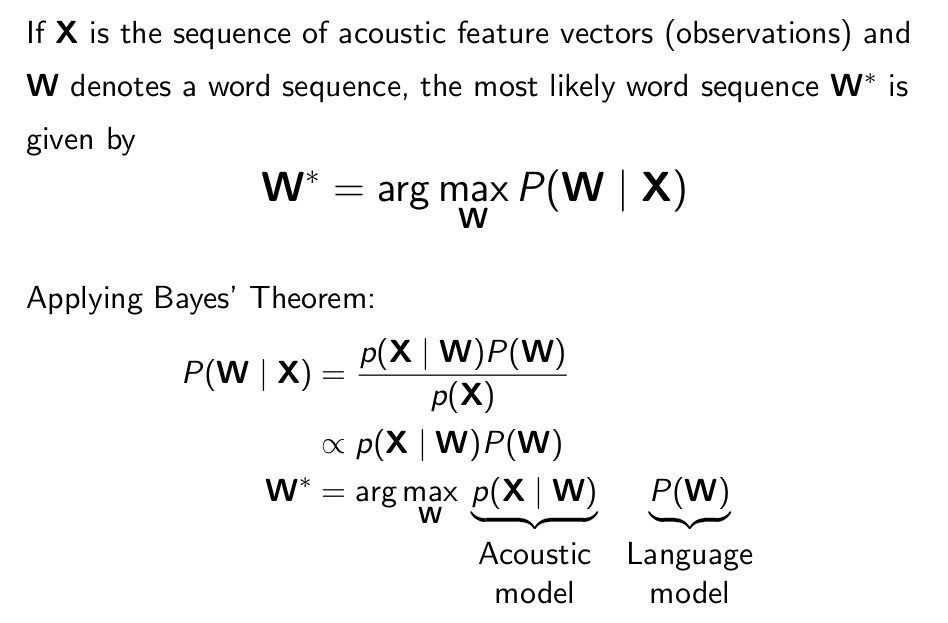
\includegraphics[scale=.33]{ASR-equations}
	\end{center}

\end{frame}

\subsection{}
\begin{frame}{Automatic speech recognition}

{\Large From the license agreement that comes with Nuance's Dragon Dictate:}
\vspace{.25cm}

\begin{alertblock}{9. Limitation of Liability}
...
LICENSEE UNDERSTANDS THAT SPEECH RECOGNITION IS A \textbf{STATISTICAL PROCESS AND THAT RECOGNITION ERRORS ARE INHERENT IN THE PROCESS}. LICENSEE ACKNOWLEDGES THAT IT IS \textbf{LICENSEE'S RESPONSIBILITY TO CORRECT RECOGNITION ERRORS BEFORE USING THE RESULTS}.
OF THE RECOGNITION.
\end{alertblock}

\end{frame}

\subsection{}
\begin{frame}{ASR Schematic Model}

	\begin{center}
    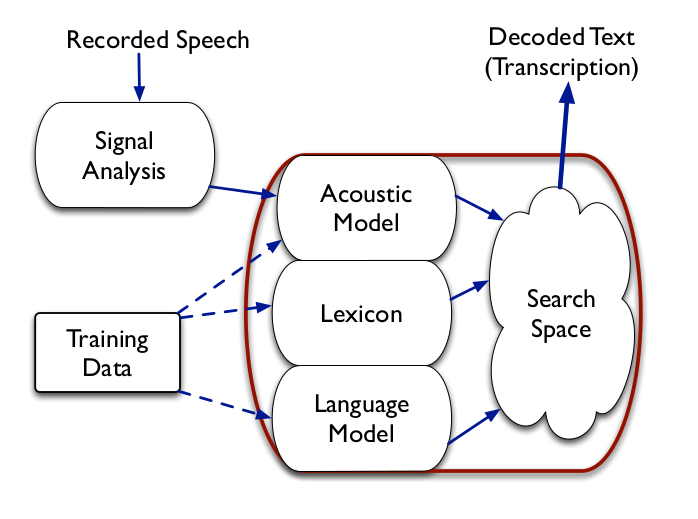
\includegraphics[scale=.4]{ASR-model}
	\end{center}
	
\end{frame}

\subsection{}
\begin{frame}{ASR Schematic Model}

	\begin{center}
    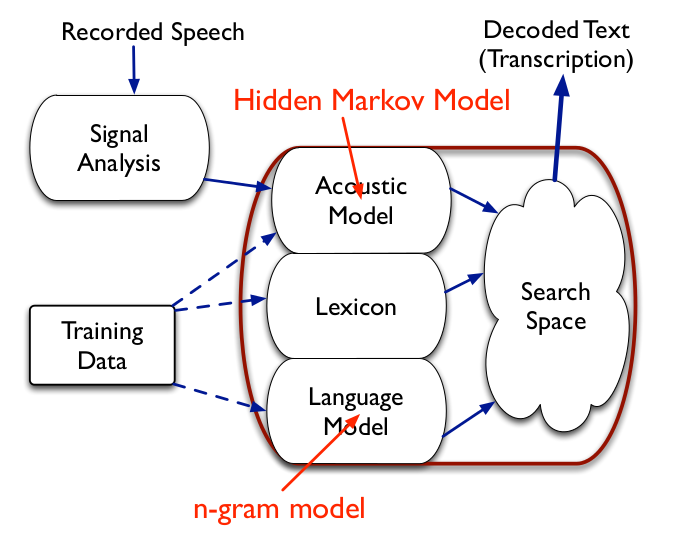
\includegraphics[scale=.4]{ASR-model2}
	\end{center}
	
\end{frame}

\subsection{}
\begin{frame}{ASR Schematic Model}

	\begin{center}
    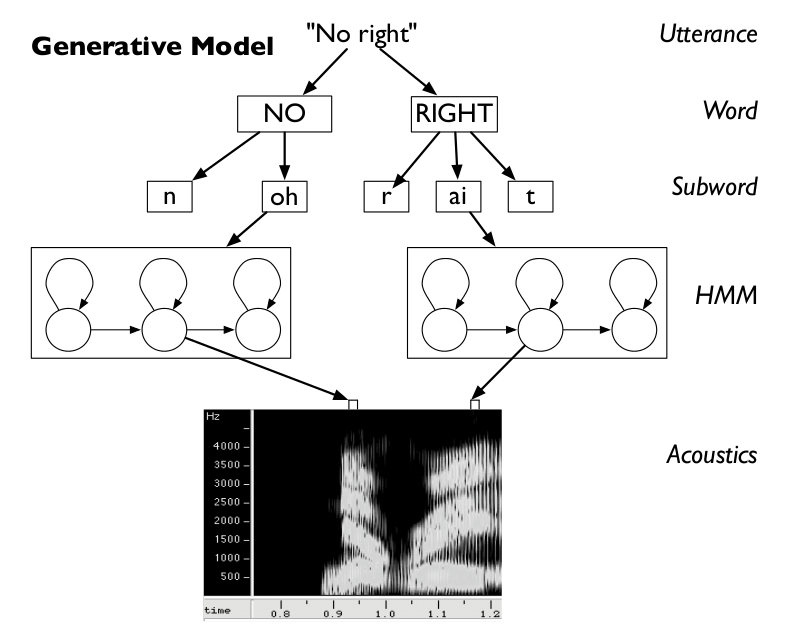
\includegraphics[scale=.35]{ASR-hierarchical}
	\end{center}
	
\end{frame}

\subsection{}
\begin{frame}{HMM for `six'}

	\begin{center}
    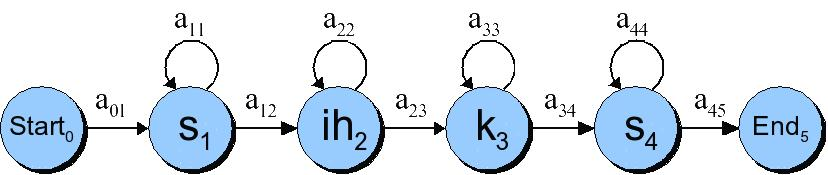
\includegraphics[scale=.3]{ASR9-6.jpg}
	\end{center}
\end{frame}

\subsection{}
\begin{frame}{Each phone has 3 states}

	\begin{center}
    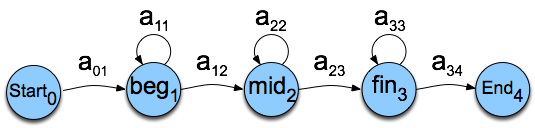
\includegraphics[scale=.5]{ASR9-6a.jpg}
	\end{center}
\end{frame}

\subsection{}
\begin{frame}{Each phone has 3 states: HMM for `six'}


    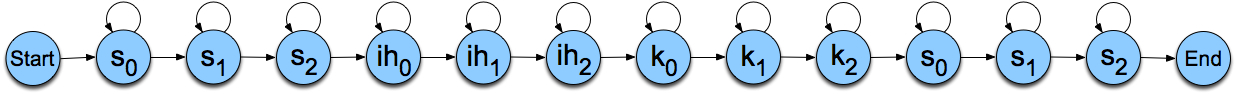
\includegraphics[scale=.26]{ASR9-7.jpg}

\end{frame}

\subsection{}
\begin{frame}{MFCC: Mel Frequency Cepstral Coefficients}


    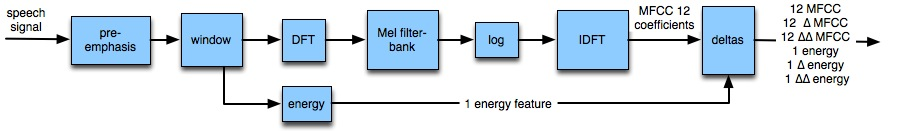
\includegraphics[scale=.38]{ASR9-8.jpg}

\end{frame}

\subsection{}
\begin{frame}{The Cepstrum}

{\large One way to think about the cepstrum:}
\begin{itemize}
	\item separating the source and filter
	\item Speech waveform is created by
	\item A glottal source waveform
	\item Passes through a vocal tract which, because of its shape, has a particular filtering characteristic 
\end{itemize}
\vspace{.25cm}

{\large Articulatory facts:}
\begin{itemize}
     \item The vocal cord vibrations create harmonics
     \item The mouth is an amplifier
     \item Depending on shape of oral cavity, some harmonics are amplified, some are dampened
\end{itemize}
\end{frame}

\subsection{}
\begin{frame}{Data!}

\begin{itemize}
	\item ASR is another example of learning from data
	\item Standard corpora with agreed evaluation protocols are very
important for the development and evaluation of ASR
	\item TIMIT corpus (1986) --first widely used corpus, still in use
	\begin{itemize}
		\item Utterances from 630 North American speakers
		\item Phonetically transcribed, time-aligned
		\item Standard training and test sets, agreed evaluation metric
(phone error rate)
	\end{itemize}
	\item Many standard corpora released since TIMIT: DARPA
Resource Management, read newspaper text (e.g, Wall St
Journal), human-computer dialogues (e.g, ATIS), broadcast
news (e.g, Hub4), conversational telephone speech (e.g. Switchboard), multiparty meetings (eg AMI)
	\item Standard corpora have most value when closely linked to evaluation
benchmark tests (with new test data from the same domain)

\end{itemize}

\end{frame}

\subsection{}
\begin{frame}{Evaluation}

\begin{itemize}
	\item How accurate is a speech recognizer?
	\item Use dynamic programming to align the ASR system's output with a reference transcription (a gold standard)
	\item Three types of error: insertion, deletion, and substitution
	\item Word error rate (\textbf{WER}), sums the three types of error.  If there
are N words in the reference transcript, and the ASR output
has S substitutions, D deletions and I insertions, then:
		\begin{equation*}WER = 100 \cdot \frac{I + D + S}{N}\%\end{equation*}
	\item Accuracy = 100 - WER\%
	\item Speech recognition evaluations: common training and development data, release of new test sets on which different systems may be evaluated using word error rate
\end{itemize}

\end{frame}

\subsection{}
\begin{frame}{For next time:}
     \begin{block}{For next time:}
          \begin{enumerate}
     	  \item Next time we'll talk in more detail about cepstral coefficients and HMMs for ASR.
     	  \item Keep reading chapter 9 of Jurafsky and Martin
     	  \item Midterm due Monday
          \end{enumerate}
     \end{block}
\end{frame}



\end{document}


